\documentclass[handout]{beamer}

\usepackage{fontspec} 
% \usepackage{lsp-makros}
\useoutertheme{lsp}

\usepackage{lsptitle}

\def\two@digits#1{\ifnum#1<10 0\fi\number#1}
\def\mytoday{\two@digits{\number\day}.\two@digits{\number\month}.\number\year}


\usepackage{xspace,multicol}
\newcommand{\latex}{\LaTeX\xspace}
\usepackage{tikz}


\newcounter{lastpagemainpart}
\footnotesep0pt
\renewcommand{\footnoterule}{}
\usefootnotetemplate{
  \noindent
  \insertfootnotemark\insertfootnotetext}

\let\beamerfn=\footnote
\renewcommand{\footnote}[1]{%
\let\oldfnsize=\footnotesize%
\let\footnotesize=\tiny%
\beamerfn<\thebeamerpauses->{#1}%
\let\footnotesize=\oldfnsize}


\date{9. Dezember 2017}

\usepackage{eurosym}  
 
\renewcommand{\centerline}[1]{\hfill#1\hfill\hfill\mbox{}}


\title{Die Community im \vphantom{j}wissenschaftlichen Publizieren}
% \institute{FU Berlin}
\author[LangSci]{Felix Kopecky, Language Science Press
% \mbox{\tiny\url{https://github.com/langsci/lsp-presentations/blob/master/oat2017books/presentation.pdf}}
}



\begin{document}
\lspbeamertitle


\section{Language Science Press}
\frame{
\frametitle{Language Science Press}
%   \includegraphics[height=.2\textheight]{./path/to/graphicsfile}
  \begin{itemize}
    \item linguistische Monographien und Sammelbände als CC-BY
    \item  aktiv seit 2014 (FU Berlin), seit 2017 HU Berlin
    \item  20 Reihen,  160 HerausgeberInnen weltweit 
    \item >45 Bücher, 300 Interessensbekundungen
    \item >250 registrierte ProofreaderInnen
    \item  911 \textit{public supporters} + 305 anonyme
    \item Plan ab 2018: 30 Bücher pro Jahr
    \item bis zu >20.000 Downloads pro Buch
  \end{itemize}
}



\section{Prinzipien}
% \subsection{Prinzip der Offenheit} 

% \subsection{Prinzip der Community}
\frame{
\frametitle{Prinzip der Community}
%   \includegraphics[height=.2\textheight]{./path/to/graphicsfile}
  ~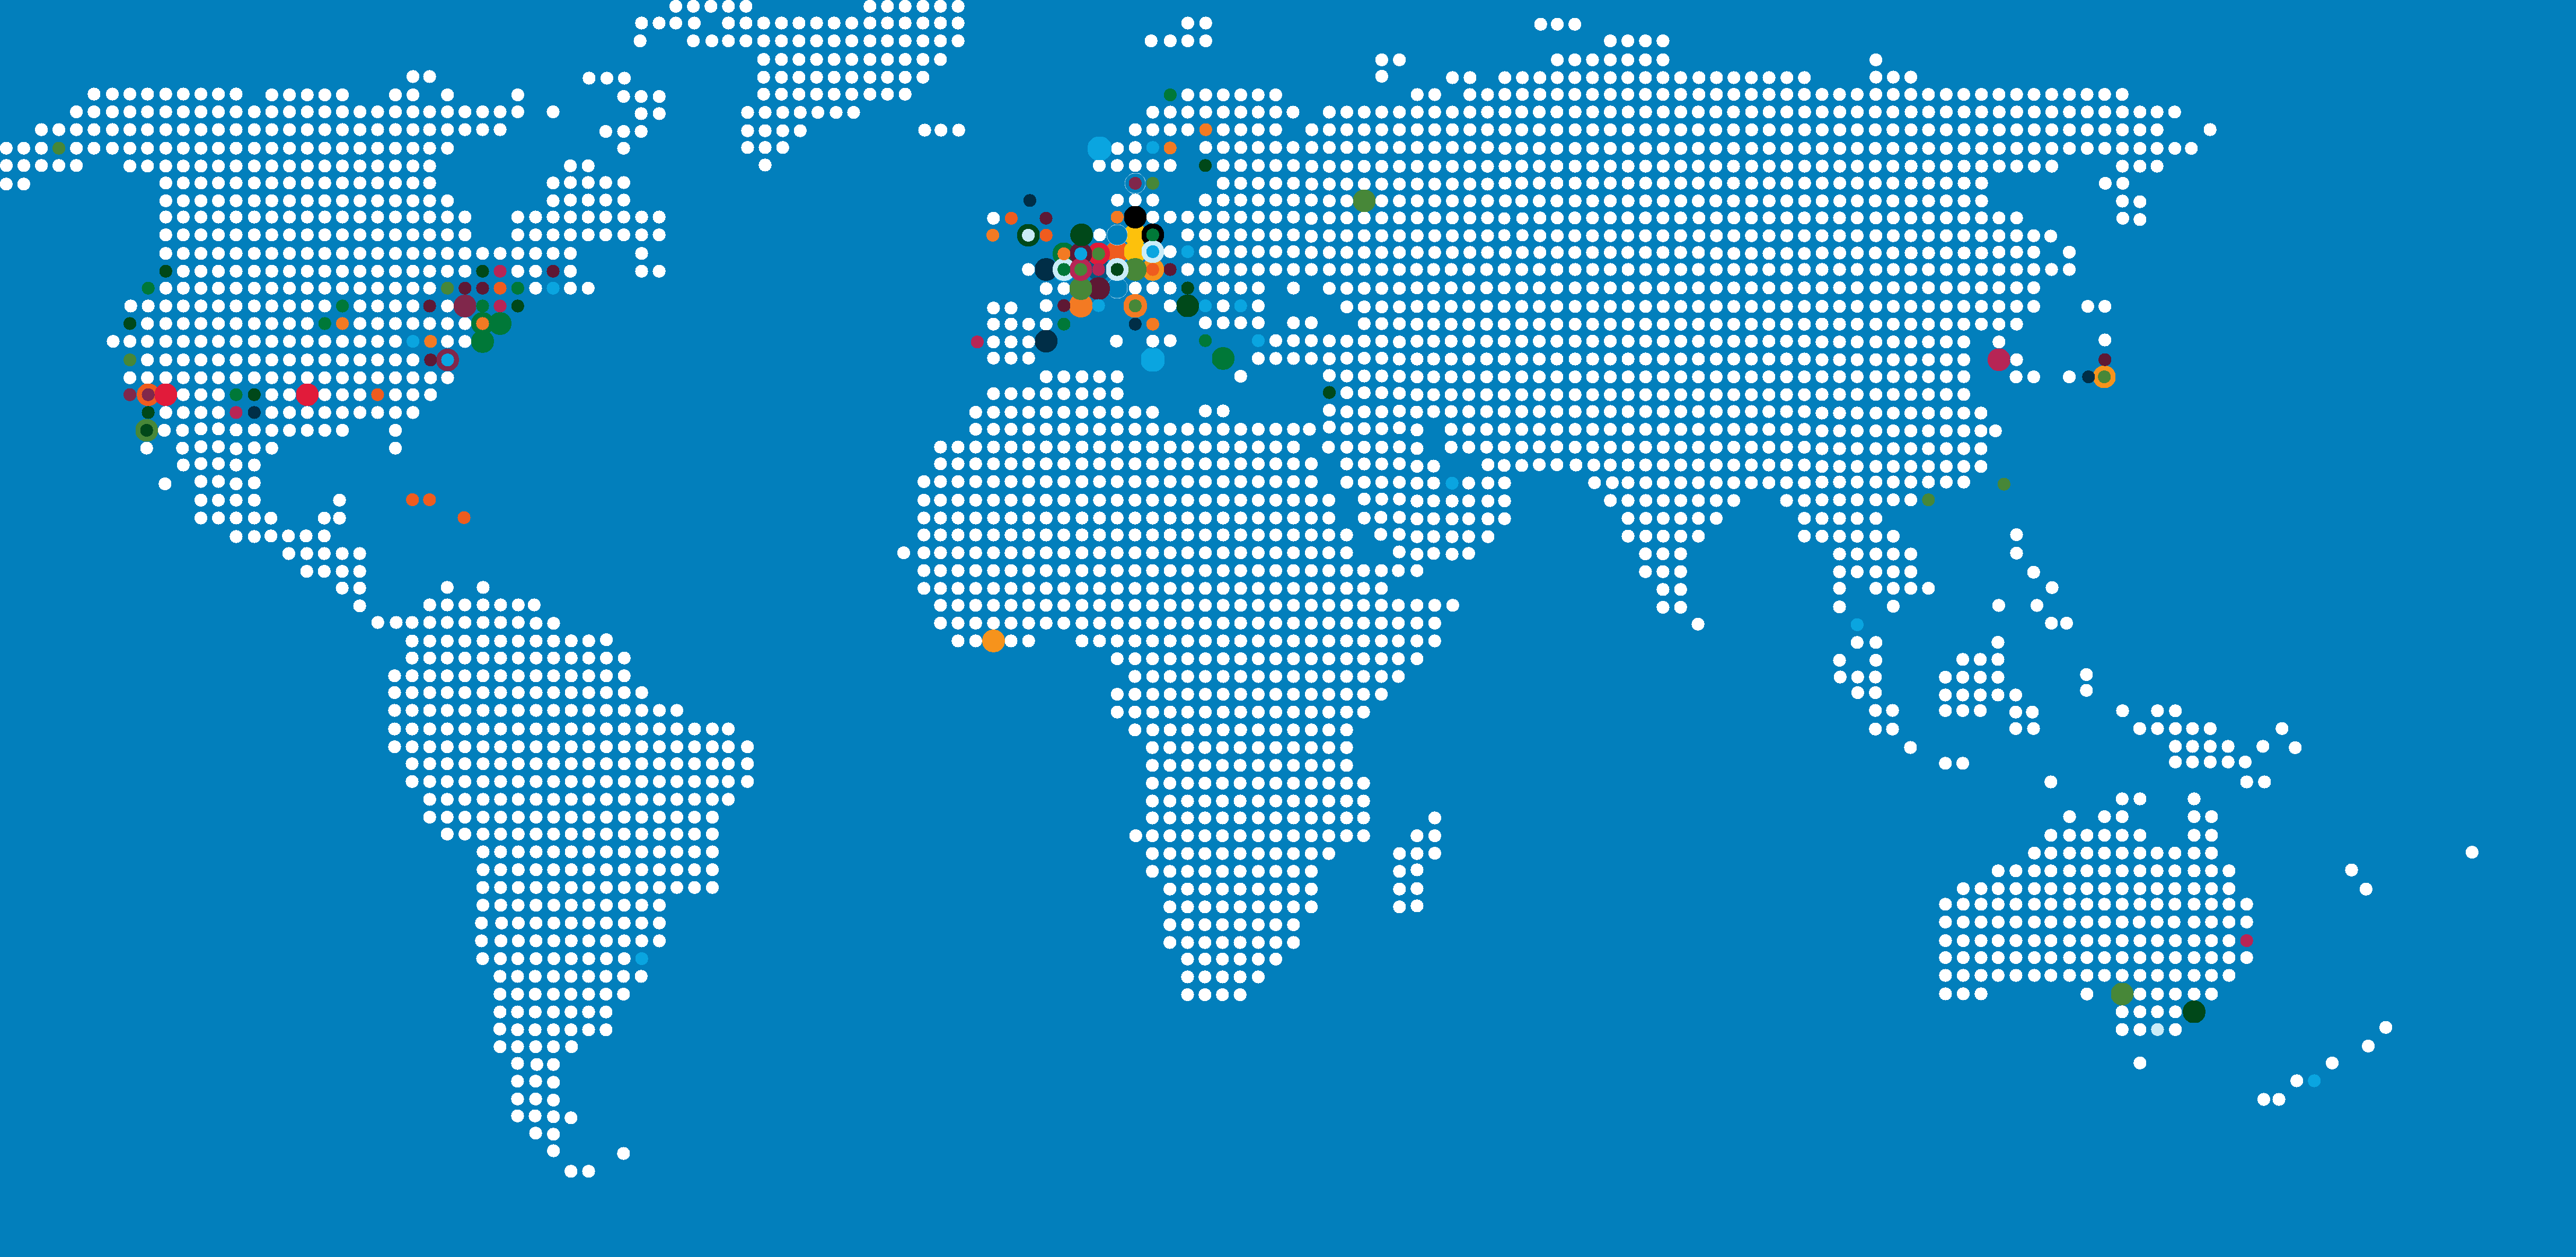
\includegraphics[width=.8\textwidth]{WORLDMAPDOTSdots.png}
  \begin{itemize}
    \item weltweit, autark, dezentral, bottom-up
    \item own the brands (Schutz vor Übernahme)
    \item share the source (Templates, Quelldateien, Kalkulationen)
    \item Anerkennungskultur
  \end{itemize}
}

\frame{
\frametitle{Prinzip der Schlankheit}
%   \includegraphics[height=.2\textheight]{./path/to/graphicsfile}
  \begin{itemize}
    \item keine Legacy-Software
    \item keine Lagerhaltung
    \item kein Vertrieb
    \item keine IT für Paywalls, Registrierung
    \item kein Marketing 
    \item keine Buchstände
    \item keine komplizierten Autorenverträge 
    \item keine Tantiemen\\$\to$ born digital
  \end{itemize}
}


\section{Umsetzung}

\frame{
\frametitle{Organisation in Reihen}
%   \includegraphics[height=.2\textheight]{./path/to/graphicsfile}
  \begin{itemize}
    \item Reihen werden von HerausgeberInnen autark verwaltet (meist namhafte ProfessorInnen mit tenure)
    \item Neue Reihen durch Advisory Board ausgewählt
    \item Qualitätskontrolle durch (open) peer review
    \item Community Proofreading: ProofreaderInnen kommen meist aus den Subcommunities unserer Reihen.
    \item 250 ProofreaderInnen bekommen alle zwei Wochen eine E-Mail mit dem jeweils aktuellen Titel
    \item Paperhive als Proofreading-Plattform
  \end{itemize}
}

\frame{ 
\frametitle{\mbox{Paperhive}}
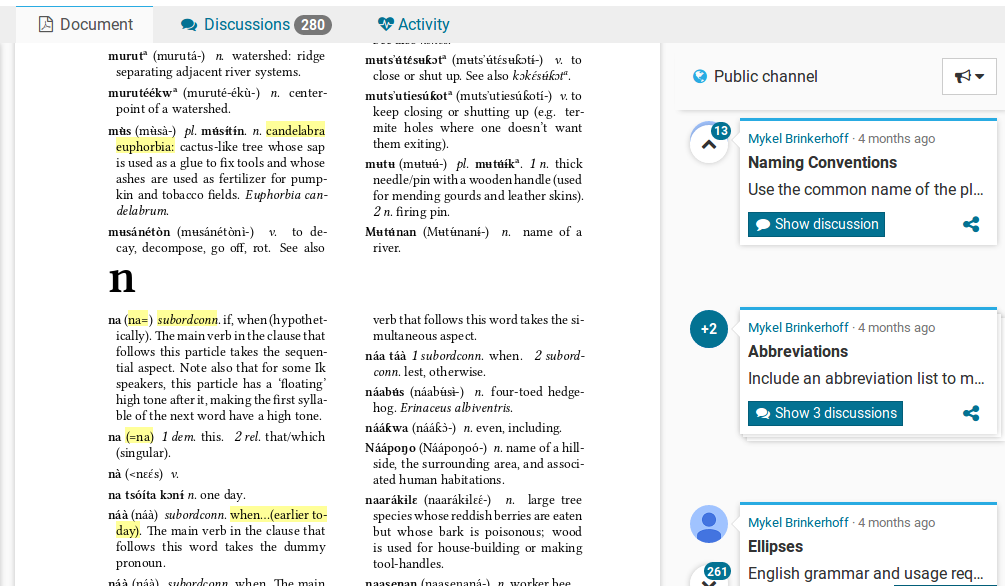
\includegraphics[height=\textheight]{communityproofreading.png}
}
 
   


% \subsection{Prinzip der Schlankheit}    

\frame{
\frametitle{Buchherstellung unter\newline AutorInnen-Einbindung}
%   \includegraphics[height=.2\textheight]{./path/to/graphicsfile}
  \begin{itemize}
    \item typographische Qualität durch \LaTeX\xspace und verpflichtende Style Rules
    \item AutorInnen haben großen Einfluss auf das fertige Buch
    \item Schwierige Elemente wie z.B. Diagramme oder Landkarten können von LangSci (nach)gezeichnet werden
    \item Schneller technischen Support
    \item Screencasts 
    \item Schnittstelle: Overleaf mit git-Einbindung
    \item Dadurch leichter Umgang selbst für technisch unerfahrene AutorInnen
  \end{itemize}
}

\frame{ 
\frametitle{\mbox{Overleaf}}
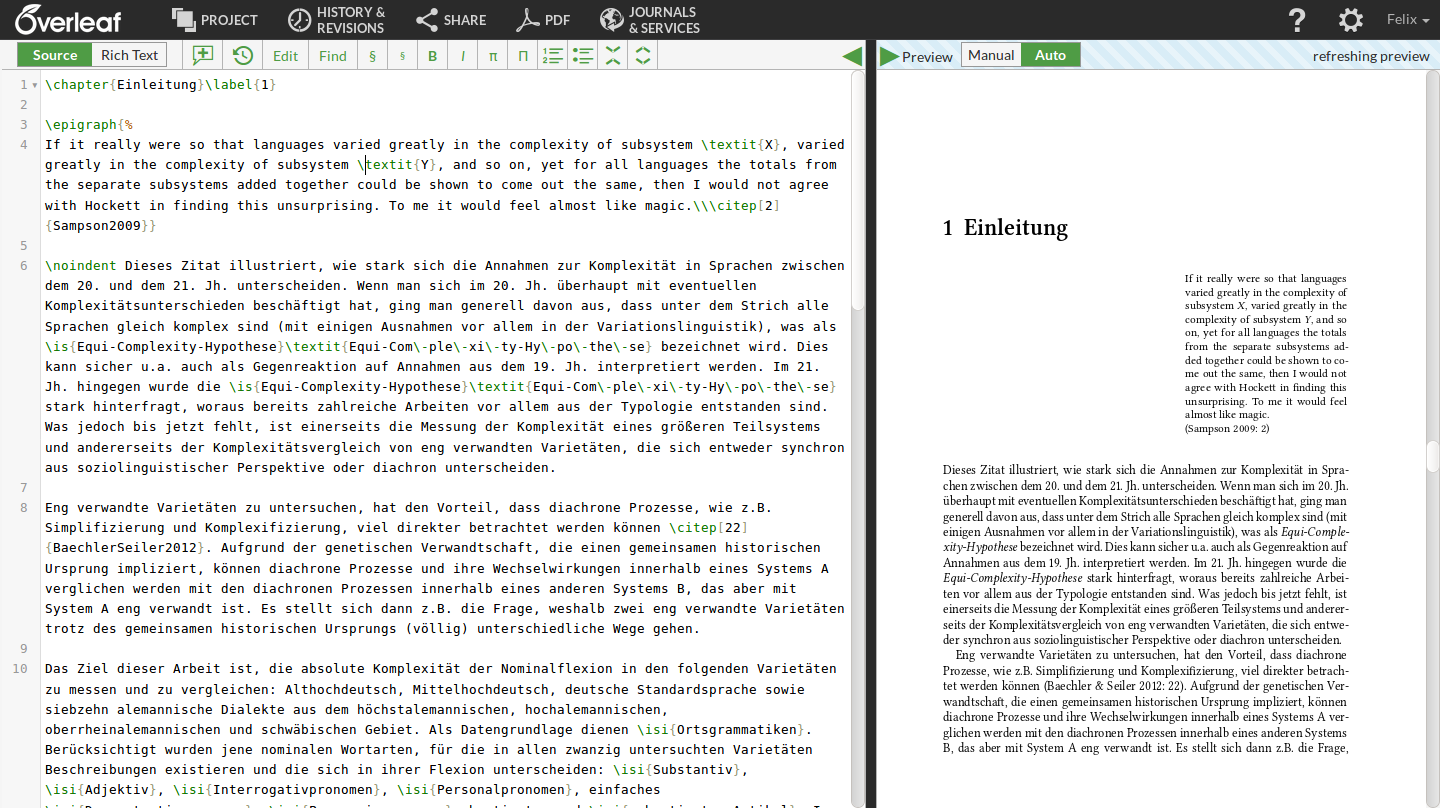
\includegraphics[height=.95\textheight]{overleaf.png}
}


% % 
% % \frame{
% % \frametitle{Voraussetzungen}
% % %   \includegraphics[height=.2\textheight]{./path/to/graphicsfile}
% %   \begin{itemize}
% %   \item Community-Building
% %   \item keine Gewinnerzielungsabsicht
% %   \item kein Anspruch auf Verwertungsrechtemonopol
% %   \item verteilte Finanzierung (konkret: Knowledge Unlatched)
% %   \item klares inhaltliches Profil
% %   \item Buchmenge überschaubar und vorhersagbar 
% %   \item Anerkennungskultur      
% %   \end{itemize} 
% % }

\end{document}